\section{Einleitung}
Die Anforderungsverwaltung (Requirements Management) wird nach dem International Requirements Engineering Board (IREB)  als einer der 4 Hauptaktivitäten im Requirements Engineering beschrieben.
% Pohl2015 S.5
Als zentrales Element steht hierbei die Sicherstellung der Verfolgbarkeit (auch:Nachvollziehbarkeit) von Anforderungen (Requirements Traceability). \cite{Pohl2015BasiswissenIREB-Standard}
% Pohl2015 S.130
Nach ISO/IEC/IEEE 29148:2011 ist eine Anforderung laut Pohl und Rupp verfolgbar,
\begin{quote}
[..] wenn sowohl der Ursprung der Anforderung als auch deren Umsetzung und die Beziehung zu anderen Dokumenten nachvollziehbar ist. \cite[S.48]{Pohl2015BasiswissenIREB-Standard}
\end{quote}
Eine so gepflegte Beziehung wird auch als Verfolgbarkeitsinformation bezeichnet. Ihre zentrale Rolle für das Requirements Management wird dadurch bestimmt, dass die Nutzung von Verfolgbarkeit allgemeine Techniken und Aspekte der Systementwicklung umfassend fördert und Vorraussetzung dafür ist, bestimmte Techniken im Entwicklungsprozess einsetzen zu können. \cite{Pohl2008RequirementsTechniken} Daher hat 
\begin{quote}
[d]ie Qualität der Nachvollziehbarkeit von Entwicklungsartefakten [..] einen großen Einfluss auf die Systementwicklung. \cite[S.507]{Pohl2008RequirementsTechniken}
\end{quote}
Die Sicherstellung der Qualität ist damit oberstes Gebot um Verfolgbarkeit gewinnbringend im Entwicklungsprozess einsetzen zu können. 

Was bedeutet aber der Begriff \enquote{Qualität} in der Requirements Traceability? Nach Gotel \& Finkelstein lässt sich Verfolgbarkeit in Pre-Requirements Specification (RS) und Post-Requirements Specification (RS) einteilen. 

\begin{figure}[!htb]
  \centering
  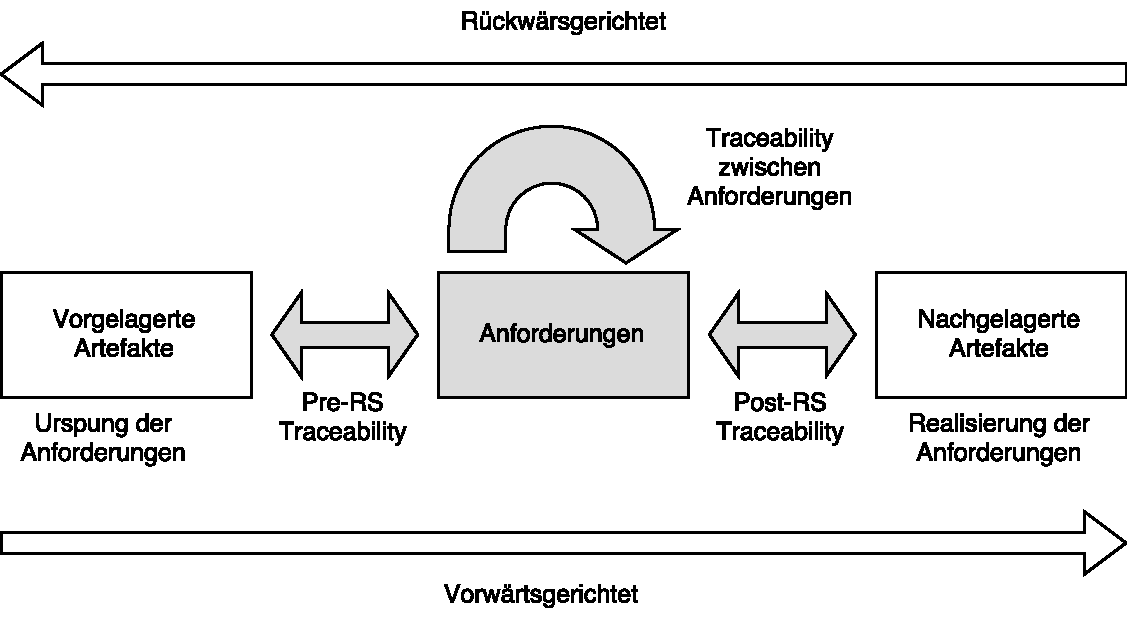
\includegraphics[width=3.5in]{PohlRupp2015_Fig_8_5.pdf}
  \caption{nach \cite[Fig. 8.5]{Pohl2015BasiswissenIREB-Standard}}
  \label{fig:abb1}
\end{figure}

Wie in \ref{fig:abb1} dargestellt wird zwischen drei Arten von Verfolgbarkeit unterschieden:

\begin{itemize}
    \item \textbf{Pre-RS:} Alle Beziehungen zu Artefakten die einer Anforderung vorgelagert sind z.B. Dokumente, Interviews etc. Im allgemeinen der Ursprung einer Anforderung
    \item \textbf{Post-RS:} Alle Beziehungen die einer Anforderung nachgelagert sind z.B Implementierung, Tests. Im allgemeinen die Auswirkung einer Anforderung
    \item \textbf{Verfolgbarkeit zwischen Anforderungen:} Abhängigkeiten oder Beziehungen zwischen Anforderungen. So kann z.B. eine Anforderung aus einem Konflikt zwischen zwei Anforderungen entstehen oder diese ersetzen. Im allgemeinen spricht man von einer Verfolgbarkeit über die Spezifikation \cite{Pohl2015BasiswissenIREB-Standard}.
\end{itemize}

Auf dem Pre-RS \& Post-RS Modell aufbauend, führt Pohl eine weitere Differenzierung ein, wie in \ref{fig:abb2} dargestellt.

\begin{figure}[!htb]
  \centering
  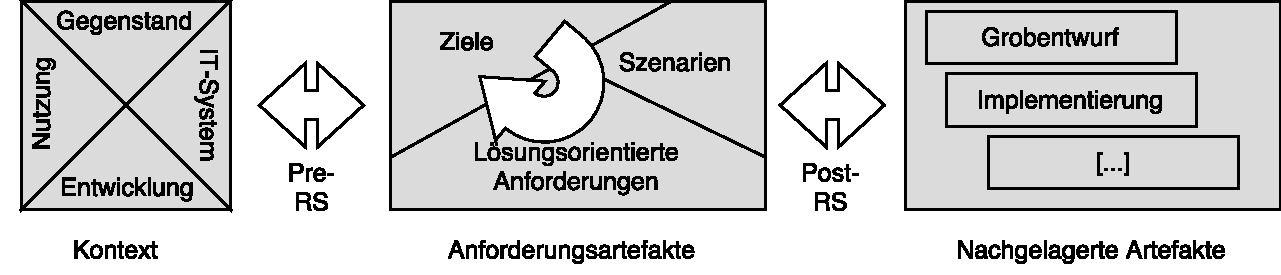
\includegraphics[width=3.5in]{Pohl2008_Fig_30_3.pdf}
  \caption{nach \cite[Fig. 30.3]{Pohl2008RequirementsTechniken}}
  \label{fig:abb2}
\end{figure}

Die \enquote{Erweiterte Pre- und Post-Traceability} präzisiert die Sicht auf die vor- und nachgelagerten Artefakte. Die Pre-RS Traceability beschreibt alle Beziehungen zwischen Anforderungsartefakten und Aspekten in einer der 4 Sichten des Systemkontext. Die Post-RS Traceability beschreibt alle Beziehungen zwischen Anforderungsartefakten und nachgelagerten Artefakten die im Entwicklungsprozess entstehen. Die Beziehung zwischen Anforderungen umfasst zusätzlich die Verfolgbarkeit zwischen Zielen, Szenarien und lösungsorientierten Anforderungen \cite{Pohl2008RequirementsTechniken}.

In \ref{fig:abb1} angedeutet wird zusätzlich zwischen \enquote{Vorwärtsgerichteter-} und \enquore{Rückwärtsgerichteter-} Verfolgbarkeit unterschieden. Um Requirements Traceability darzustellen benötigt es also einer Verfolgbarkeit zwischen Anforderungen wie auch zu ihren vorgelagerten und nachgelagerten Artefakten. Diese Verbindung muss Bidirektional sein, d.h. die Verfolgbarkeit muss von der Quelle bis zur Realisierung und Umgekehrt möglich sein. Weiterhin sind 


%Eine gute Qualität von Traceability kann nur dann gewährleister werden, wenn folgende Bedingungen gelten

%\begin{itemize}
    %\item[Projektspezifische Gestaltung] Die Aufzeichnung aller Traces ist auf Grund von wirtschaftlichen Gründen und zeitlichen Rahmenbedingungen in der Praxis nicht vertretbar. Aus diesem Grund ist eine systematik notwendig die den Gegegebenheiten und Zielsetzungen des Projekts entsprechen.
%\end{itemize}

Mit Qualität meint man im allgemeinen die Vollständige, Konsistente und Fehlerfreie pflege von Traces.


% allgemein traceability, forward, backward, pre-rs- post-rs, between, unterstützung

% wo will ich hier hin?
%Im Projekt gestaltet sich die Aufzeichnung aller denkbaren Traces auf Grund von wirtschaftlichen wie zeitlichen Rahmenbedingungen als kaum vertretbar. Daher ist die Entwicklung einer projektspezifischen Systematik notwendig die den Gegebenheiten und Zielsetzungen entsprechen \cite{Pohl2008RequirementsTechniken}. Im Umkehrschluss kann dies aber auch bedeuten, das Nachvollziehbarkeitsinformationen auf Grund von zu hohem Zeit- oder Kostenaufwand nicht erfasst werden, die anderweitig hätten gewinnbringend verwendet werden können. Daher ist es vom großen Interesse die benötigten Resourcen zu minimieren um sie mit vertretbarem Aufwand einsetzen zu können.



